\chapter{Results}
\label{chap:phages_results}

This chapter first presents the outcomes of our model in well-mixed chemostat environments, before focusing on a spatially structured environment, showing traveling wave dynamics. In these environments we observe a protective effect for phage-sensitive bacteria due to the presence of phage-resistant bacteria. This effect is further investigated and we are able to show that the effect results from a decoupling of phage and bacterial front, resulting in a widening of the peak of phage-sensitive bacteria in the system. Comparing the scenario to a similar scenario without phage-resistant bacteria, we observe a stark difference in the strength of the effect, letting us conclude that phage-resistant bacteria are necessary to observe the effect.

\section{Chemostat observations}
First we study the system in a well-mixed, chemostat environment with initial conditions given in table~\ref{tab:initial_conditions}. As expected, when increasing the dilution rate in a chemostat with only sensitive bacteria, we observe a monotonic decline in the amount of sensitive bacteria in a steady state in the chemostat~(Figure~\ref{fig:results_chemostat_traveling_wave}a, black curve). When adding phages, we observe an overall decline in sensitive bacteria. When the dilution rate is low, there are significantly less sensitive bacteria. In contrast to the sensitive only scenario, the amount of sensitive bacteria increases with increasing dilution rate up to a point where it is identical to this scenario. Then it declines in the same pattern with increasing dilution rate~(Figure~\ref{fig:results_chemostat_traveling_wave}a, red curve). This indicates a lower wash out rate for phages than for sensitive bacteria. Lastly, when adding resistant bacteria with equal fitness to the system, we observe a similar pattern but the amount of sensitive bacteria is lower at any point, indicating the competition over nutrients with resistant bacteria~(Figure~\ref{fig:results_chemostat_traveling_wave}a, blue curve). The peak of sensitive bacteria is reached at a lower dilution rate than without resistant bacteria. Choosing now the dilution rate at this peak, we study the change of sensitive bacteria when changing the fitness of the resistant bacteria in the system. We observe sensitive bacteria in the system for resistant fitness values lower than equal fitness and then a sharp decline at equal fitness~(Figure~\ref{fig:results_chemostat_traveling_wave}b, blue curve). This shows that resistant bacteria outcompete sensitive bacteria in a well-mixed environment as described previously~\cite{Levin1977-lz, Han2012-jp} and observed experimentally~\cite{Lenski1985-wb, Levin1977-lz, Spus2023-jv}.
\begin{figure}
\centering
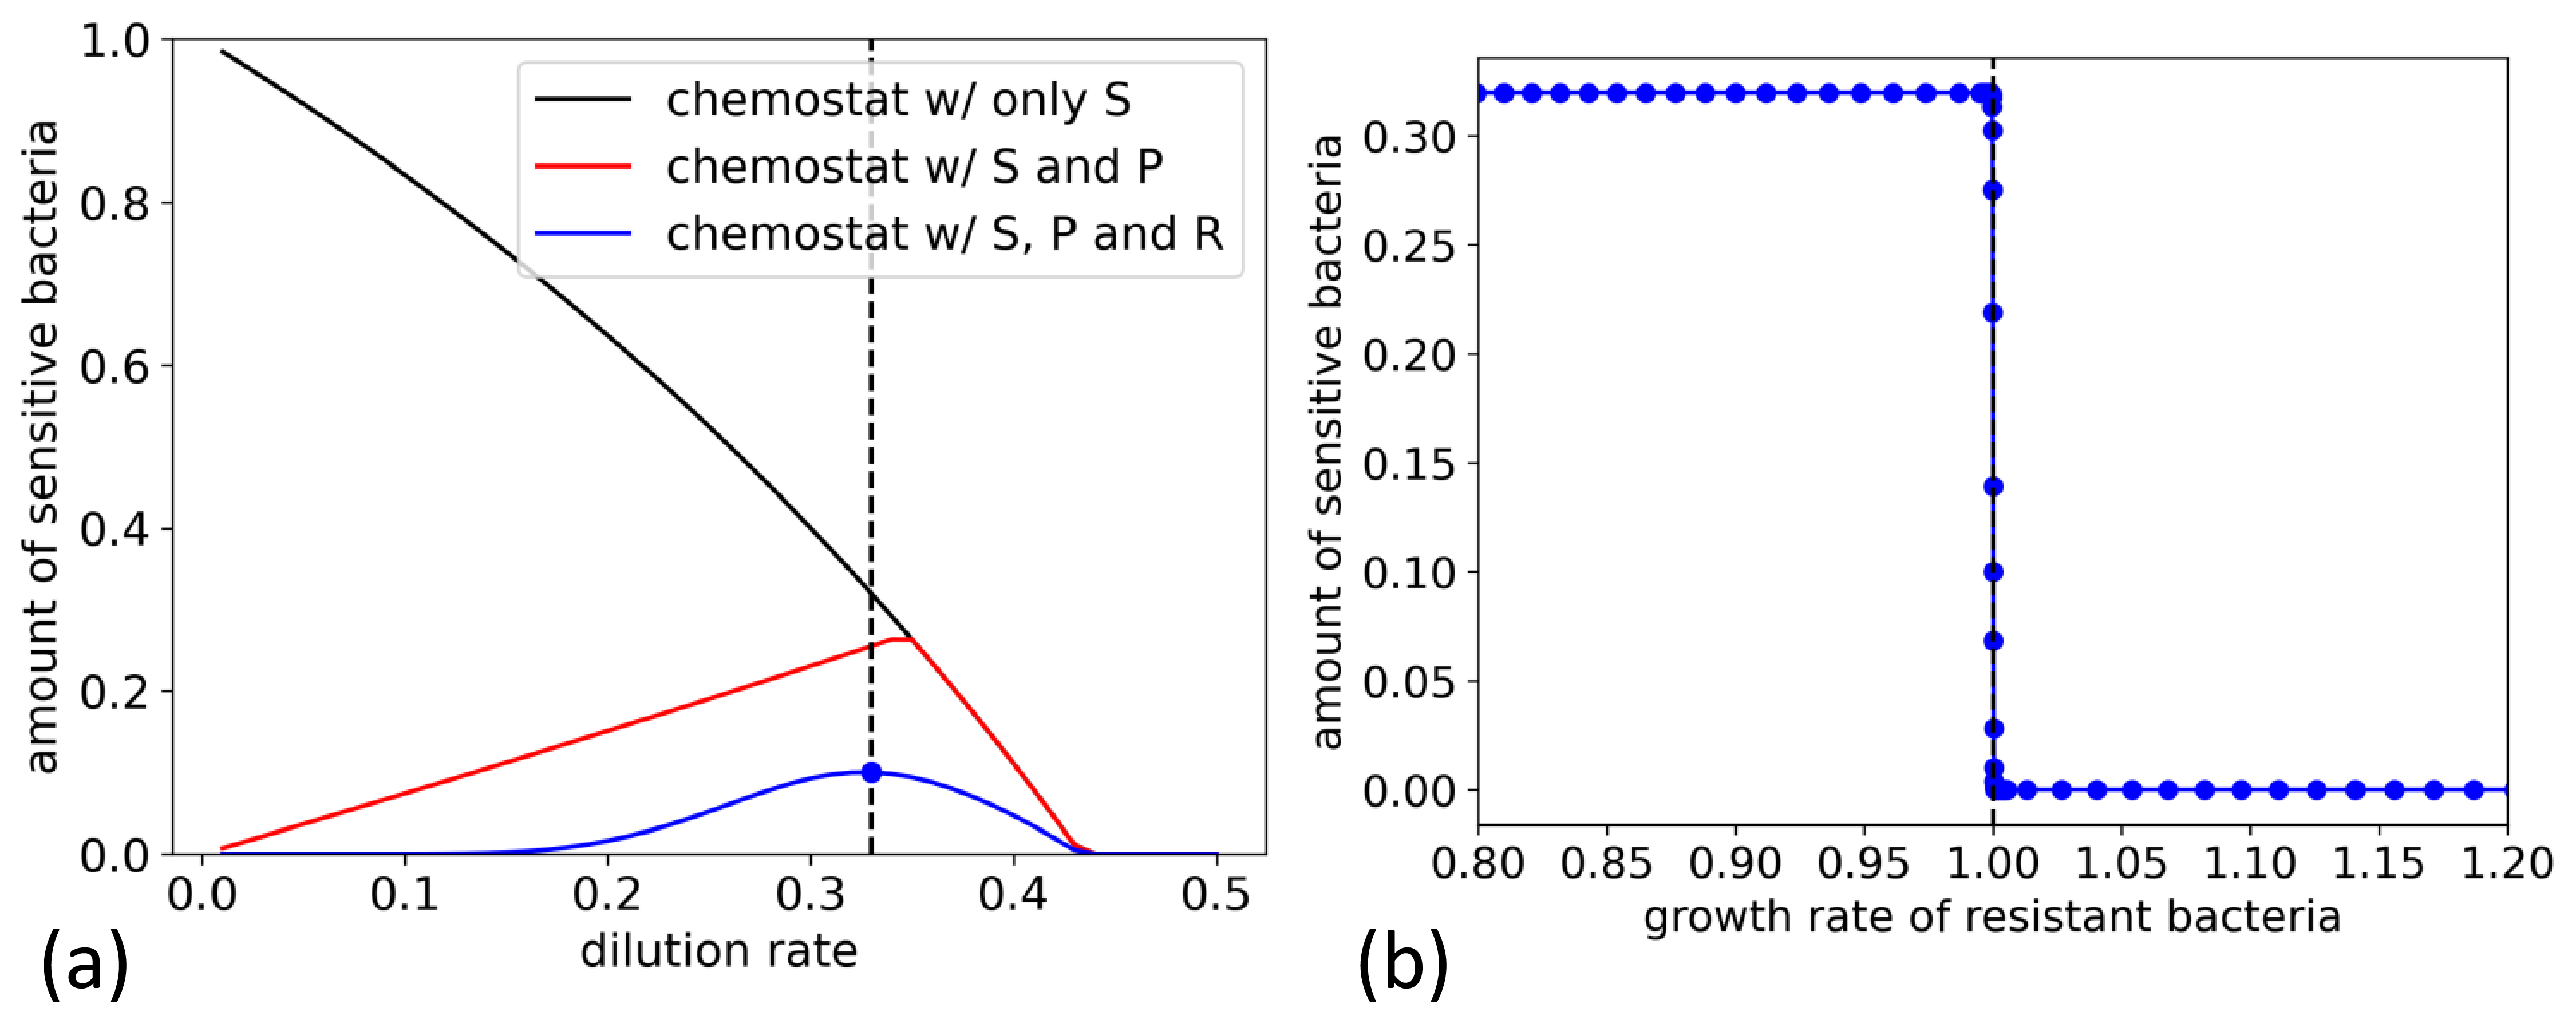
\includegraphics[width=\linewidth]{graphics/2025_09_30_phages_fig3.png}
\caption{\textbf{Resistant bacteria outcompete sensitive bacteria in a chemostat} (a) shows the amount of sensitive bacteria depending on the dilution rate for different scenarios. In black is a scenario with only sensitive bacteria, in red a scenario with phages and sensitive bacteria and in blue a scenario with phages, sensitive and resistant bacteria with $\lambda_r=1.0$. The point and dashed line indicate the optimal dilution rate $d_{max} = 0.33$ with the highest amount of sensitive bacteria when competing with resistant bacteria. (b) shows the amount of sensitive bacteria changing with the growth rate of resistant bacteria for a chemostat with dilution rate $d_{max} = 0.33$. The chemostat shows a sharp decline of sensitive bacteria at the point of equal fitness of resistant and sensitive bacteria. This indicates that sensitive bacteria go extinct ones resistant bacteria are fit enough to take over.}
\label{fig:results_chemostat_traveling_wave}
\end{figure}

\begin{table}
    \centering
    \begin{tabular}{c|c|c}
         component & chemostat & one-dimensional \\ \hline
         $S(x,0)$& 0.5 & 0.5 for x = 0, else 0.0 \\ 
         $I(x,0)$& 0.0 & 0.0 for all x\\ 
         $R(x,0)$& 0.5 & 0.5 for x = 0, else 0.0 \\
         $P(x,0)$& 1.0 & 1.0 for x = 0, else 0.0 \\
         $n(x,0)$& 1.0 & 1.0 for all x \\
    \end{tabular}
    \caption{Initial conditions used to solve the model}
    \label{tab:initial_conditions}
\end{table}

\section{Traveling wave dynamics}
Switching now from a well-mixed, liquid, chemostat environment to a one-dimensional environment with diffusion of bacteria, phages and nutrients, we simulate the system at two points, with low resistant growth rate ($\lambda_r \approx 0.617$) and with high resistant growth rate ($\lambda_r \approx 1.13$). In both cases we use initial conditions given in table~\ref{tab:initial_conditions}. For both scenarios, we obtain traveling wave dynamics, where bacteria travel through the system, invading previously unoccupied regions. The nutrients are consumed and form a receding wave, allowing a bacterial front to be formed. Time series for both scenarios are shown in Figure~\ref{fig:traveling_wave_dynamics}. As expected, the front for low resistant growth rate is mostly composed of sensitive bacteria (Figure~\ref{fig:traveling_wave_dynamics}a, blue curve) with a shallow resistant front following (Figure~\ref{fig:traveling_wave_dynamics}a, brown curve). Trailing behind is a phage front (Figure~\ref{fig:traveling_wave_dynamics}a, orange curve) which restricts the sensitive bacteria to a narrow region between its front and the phage front. In a narrow intermediate region, a small peak of infected bacteria forms (Figure~\ref{fig:traveling_wave_dynamics}a, pink curve). The shallow resistant front travels unimpeded by phages through the system. Focusing now on the second scenario, we observe, like in the chemostat scenario, that resistant bacteria take over the front, leading to rapid extinction of the sensitive bacteria (Figure~\ref{fig:traveling_wave_dynamics}b). If we track the amount of sensitive bacteria in the system over time for these two scenarios (Figure~\ref{fig:protective_effect}b, green and pink curves), we observe for low resistant growth rate scenario (green curve) that a fixed amount is being reached after an initialization phase, describing the formation of a quasi steady state of the system. For the high resistant growth rate scenario (pink curve), we see rapid extinction of sensitive bacteria, describing the observed takeover of the population by resistant bacteria as expected due to the growth advantage.

\begin{figure}
\centering
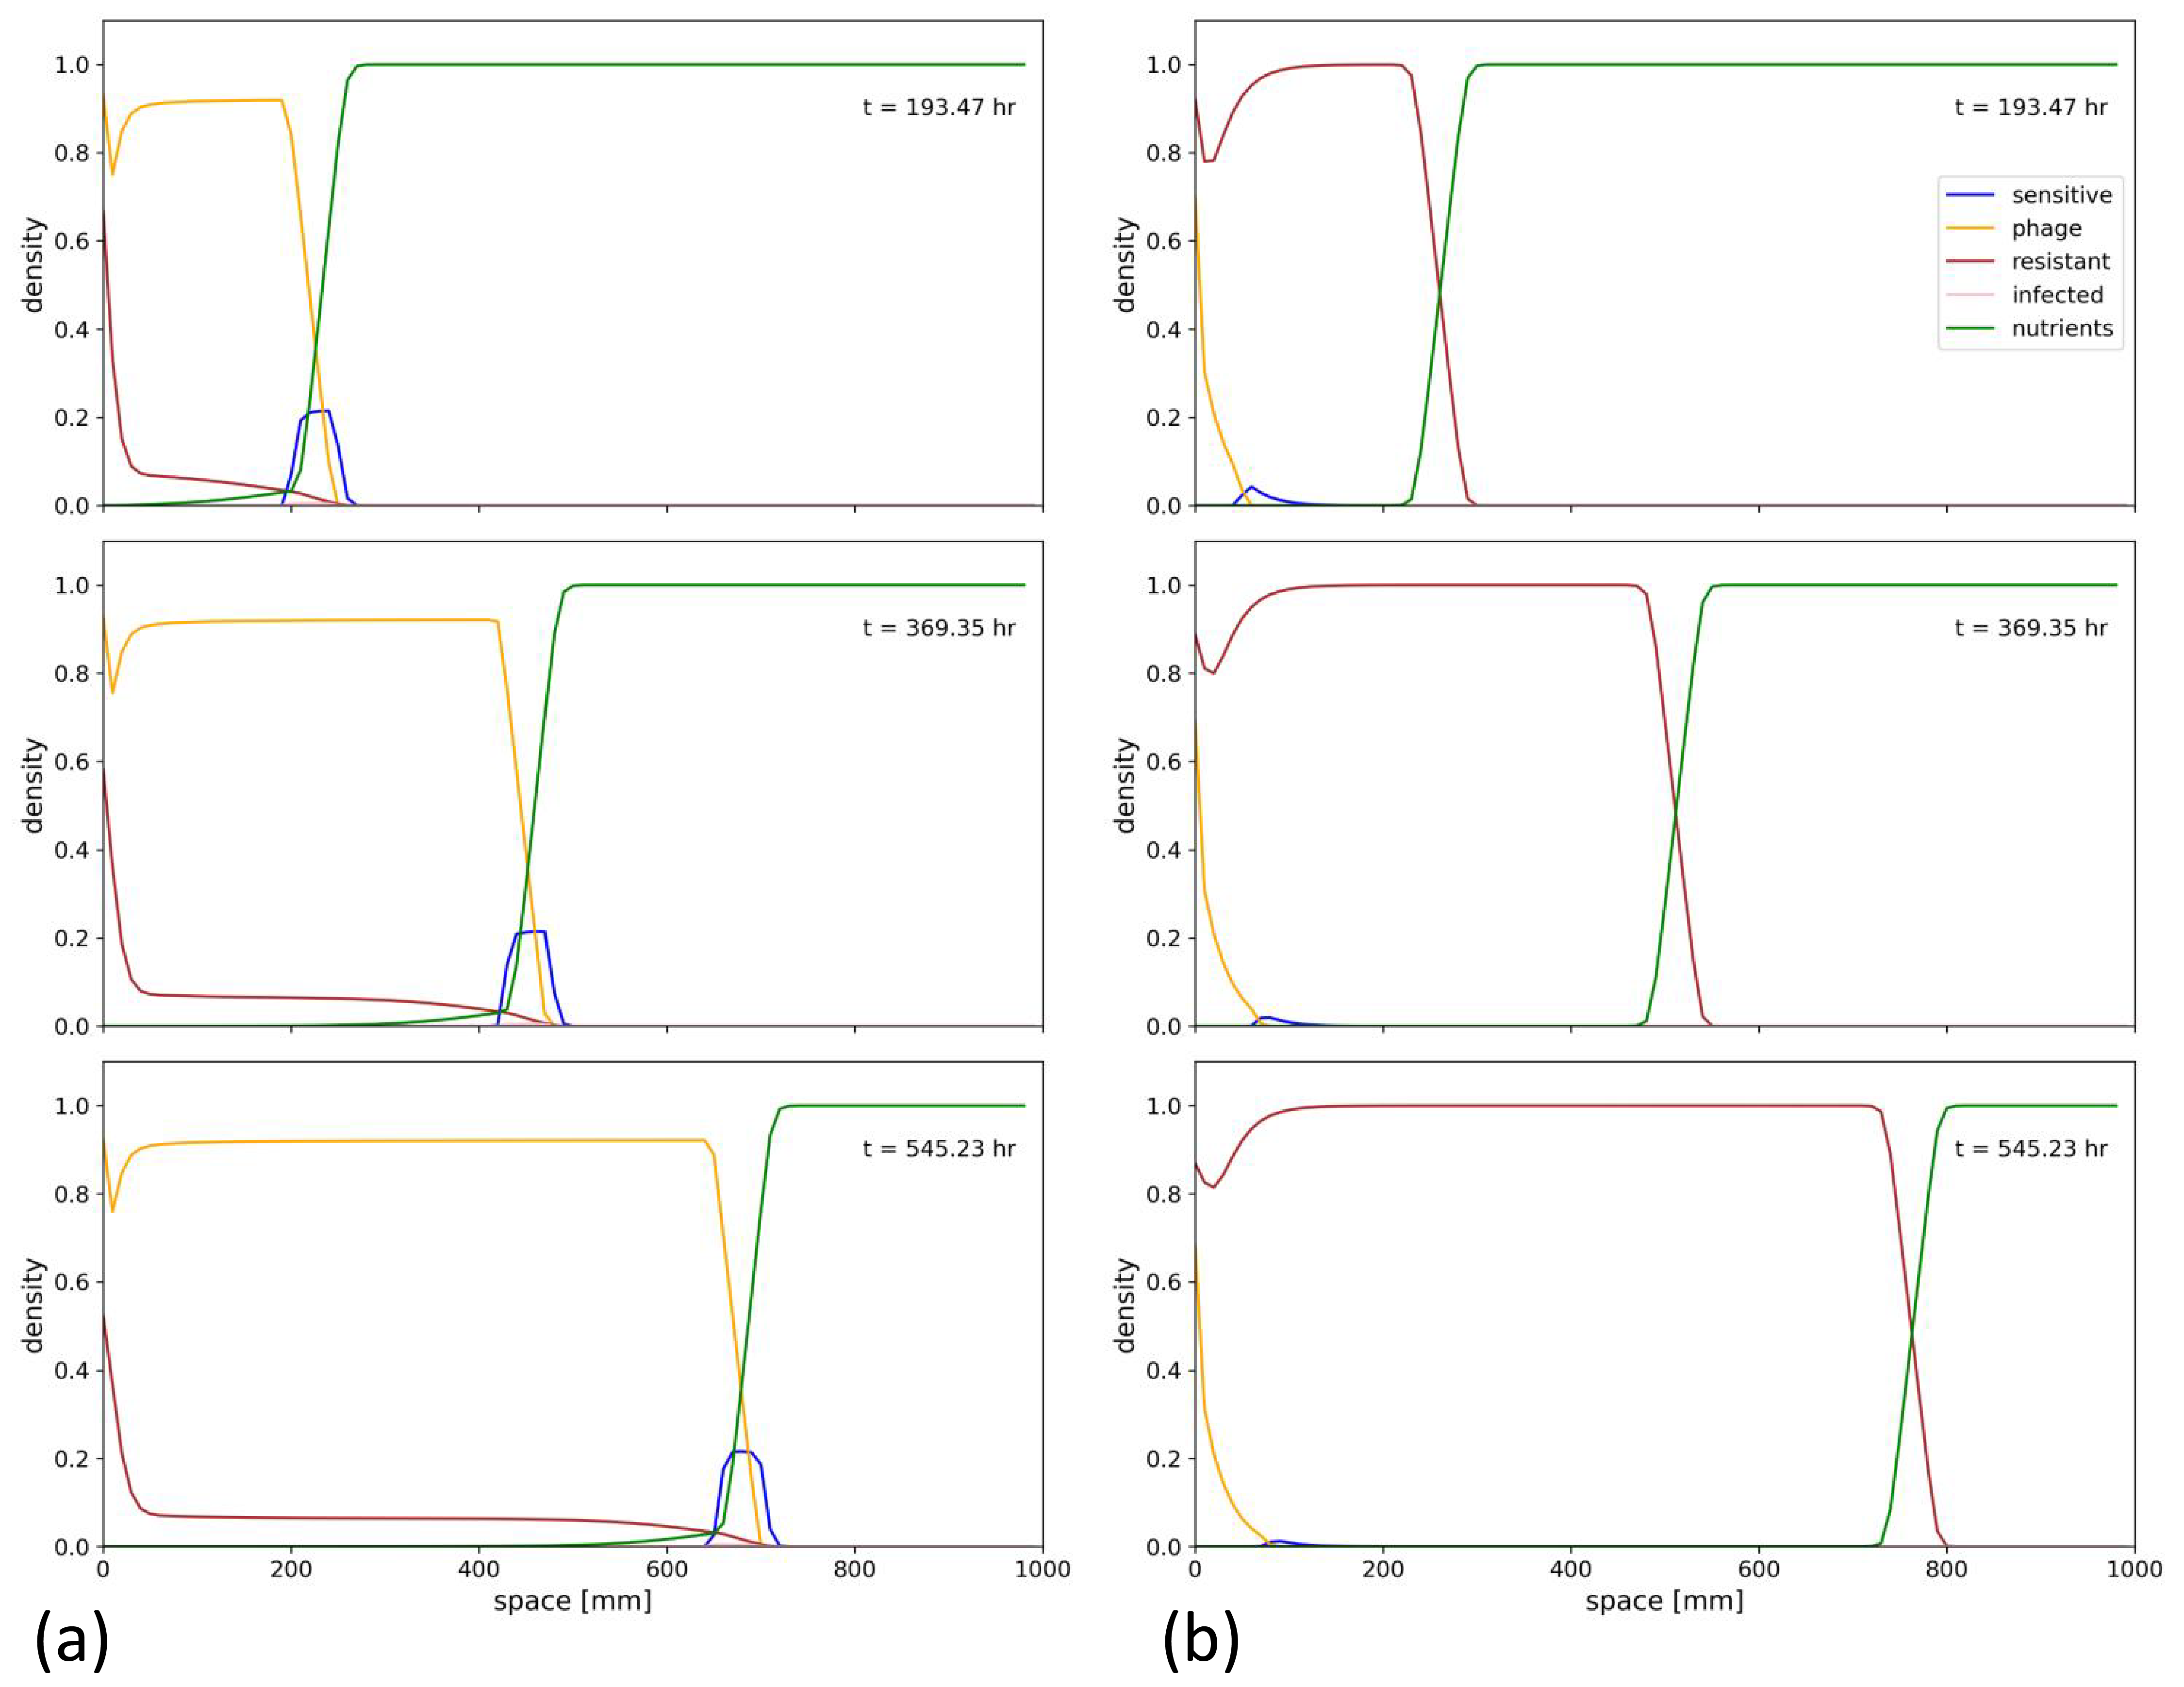
\includegraphics[width=\linewidth]{graphics/2025_09_30_phages_fig4.png}
\caption{\textbf{Traveling wave dynamics for low $\lambda_r$ and high $\lambda_r$ show survival and extinction of sensitive bacteria} This figure shows two snapshots of the dynamics formed when solving the model for different $\lambda_r$ with different outcomes. (a) shows a scenario with $\lambda_r \approx 0.617$ , revealing the survival of a traveling sensitive wave which propagates ahead of a phage wave and a shallow wave of resistant bacteria. Where phages caught up, infected bacteria are formed but they do not reach the sensitive front. (b) shows a scenario with $\lambda_r \approx 1.13$ , revealing the overtake of the system by resistant bacteria and due to nutrient exhaustion, phages and sensitive bacteria are not able to propagate and they slowly go extinct.}
\label{fig:traveling_wave_dynamics}
\end{figure}

\section{Protection by resistant bacteria}
\label{sec:protective_effect}
In the chemostat scenario, we see a rapid transition from a fixed sensitive amount to extinction at equal growth rates. Surprisingly, when simulating the system in one dimension close to this expected transition point, we see an increase in amount of sensitive bacteria just below the expected transition point while above sensitive bacteria go extinct as expected (Figure~\ref{fig:protective_effect}a, red curve). As this increase depends on the resistant growth rate, we assume it to be a protective effect for the sensitive bacteria, mediated by resistant bacteria. When studying the change of the amount of sensitive bacteria over time for the maximum of this peak (Figure~\ref{fig:protective_effect}b, black curve), we observe a constant, linear increase of amount of sensitive bacteria over time, in contrast to the two other previously studied scenarios (Figure~\ref{fig:protective_effect}b, green and pink curves).

\begin{figure}
\centering
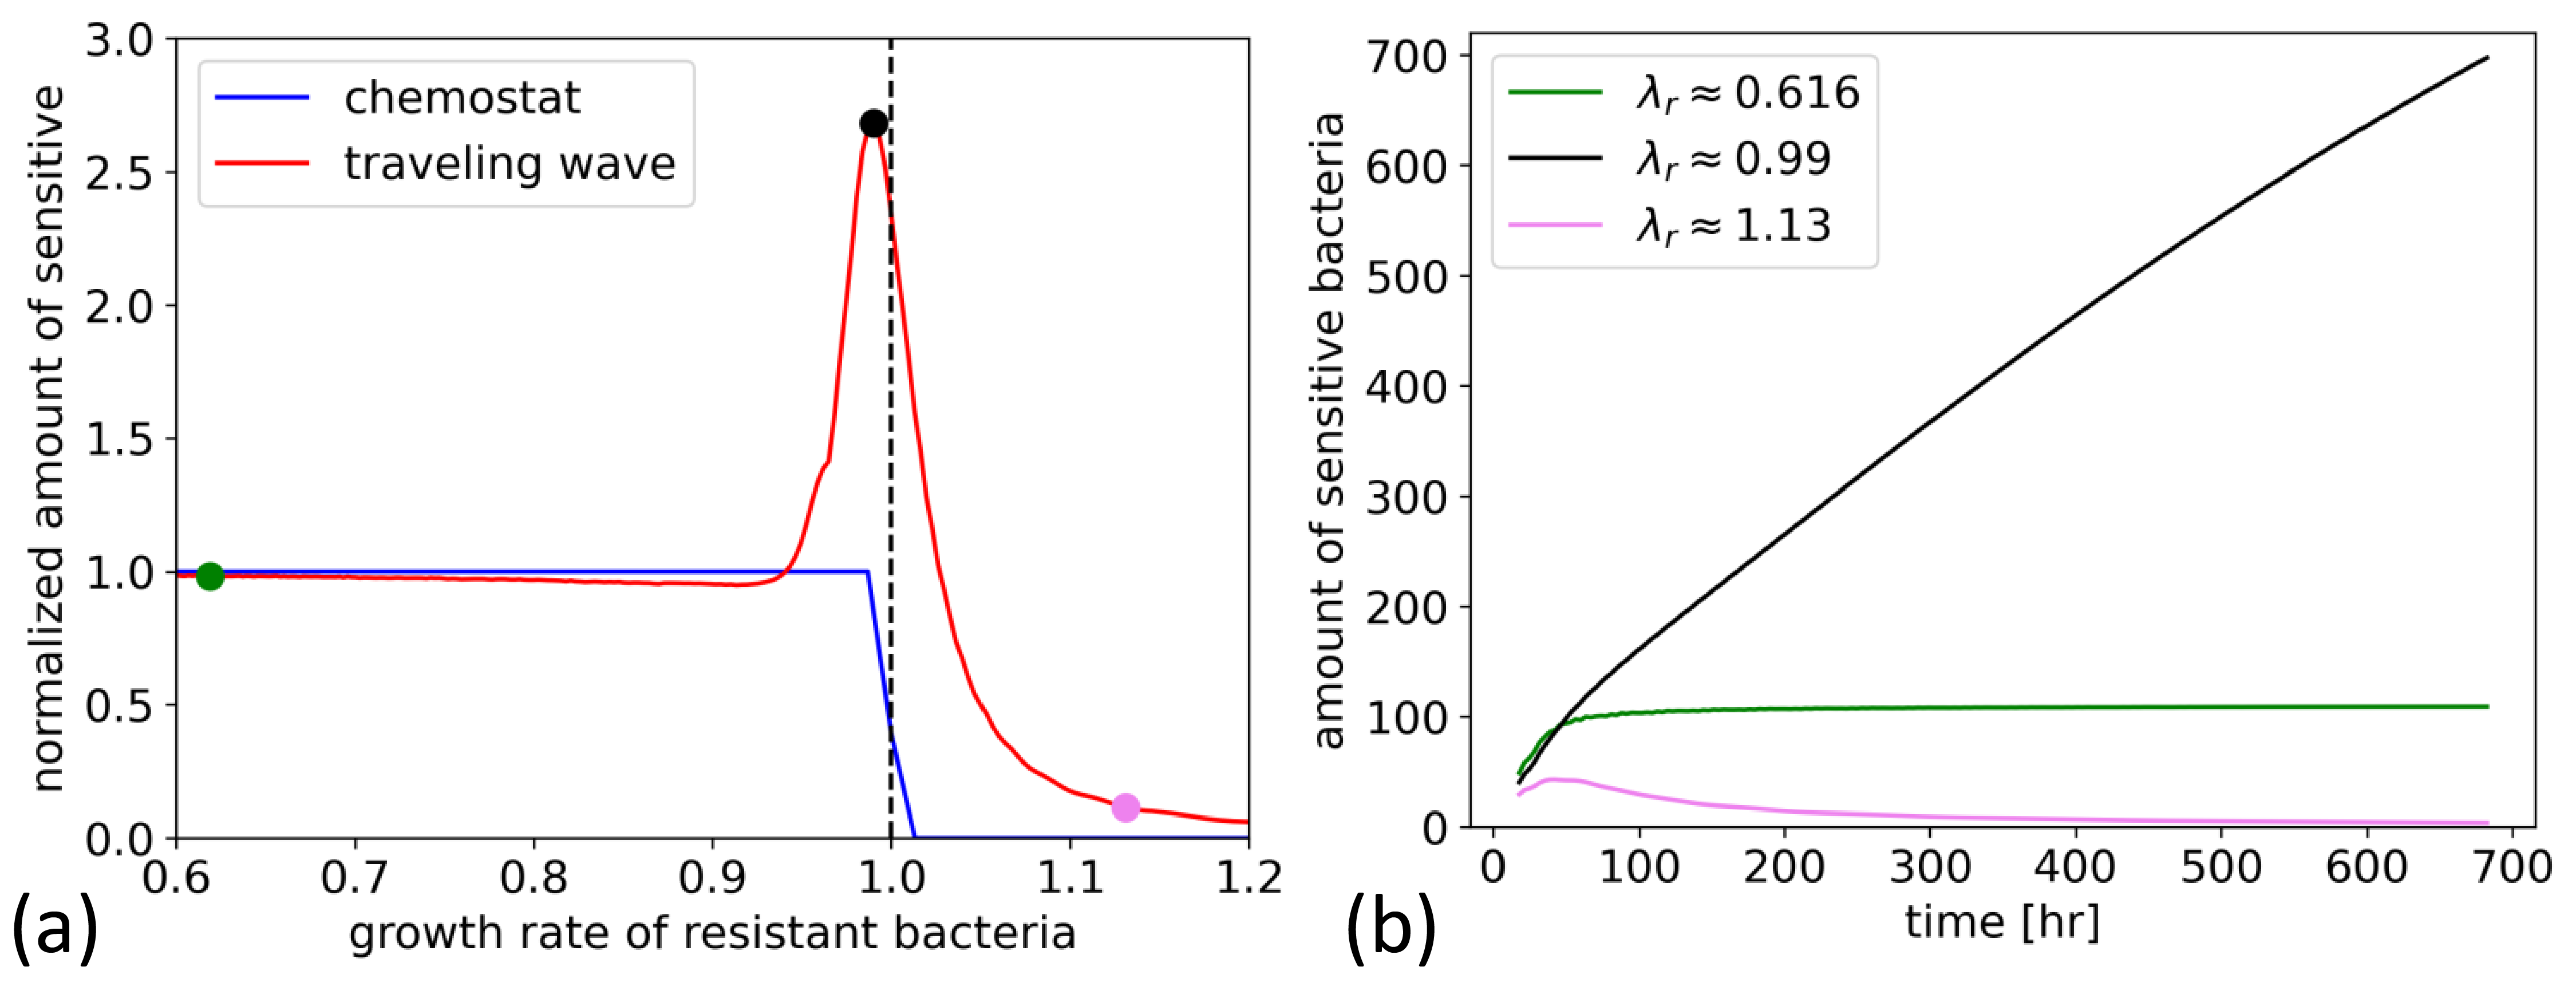
\includegraphics[width=\linewidth]{graphics/2025_09_30_phages_fig5.png}
\caption{\textbf{Resistant bacteria protect sensitive bacteria in a structured environment} (a) shows the comparison between a chemostat and the one-dimensional traveling wave scenario in a spatially structured environment. The traveling wave scenario reveals a protective effect resulting in an increase in sensitive bacteria just before the point of equal fitness of resistant and sensitive bacteria. When resistant bacteria grow faster, sensitive bacteria go extinct. The colored markers indicate the points for which we present the dynamics in Figure~\ref{fig:traveling_wave_dynamics} and in Figure~\ref{fig:dynamics_peak}. (b) shows the amount of sensitive bacteria at those chosen points over time, indicating plateauing for low resistant growth rates, continuous increase for the peak of the protective effect and extinction for high resistant growth rates.}
\label{fig:protective_effect}
\end{figure}

\begin{figure}
\centering
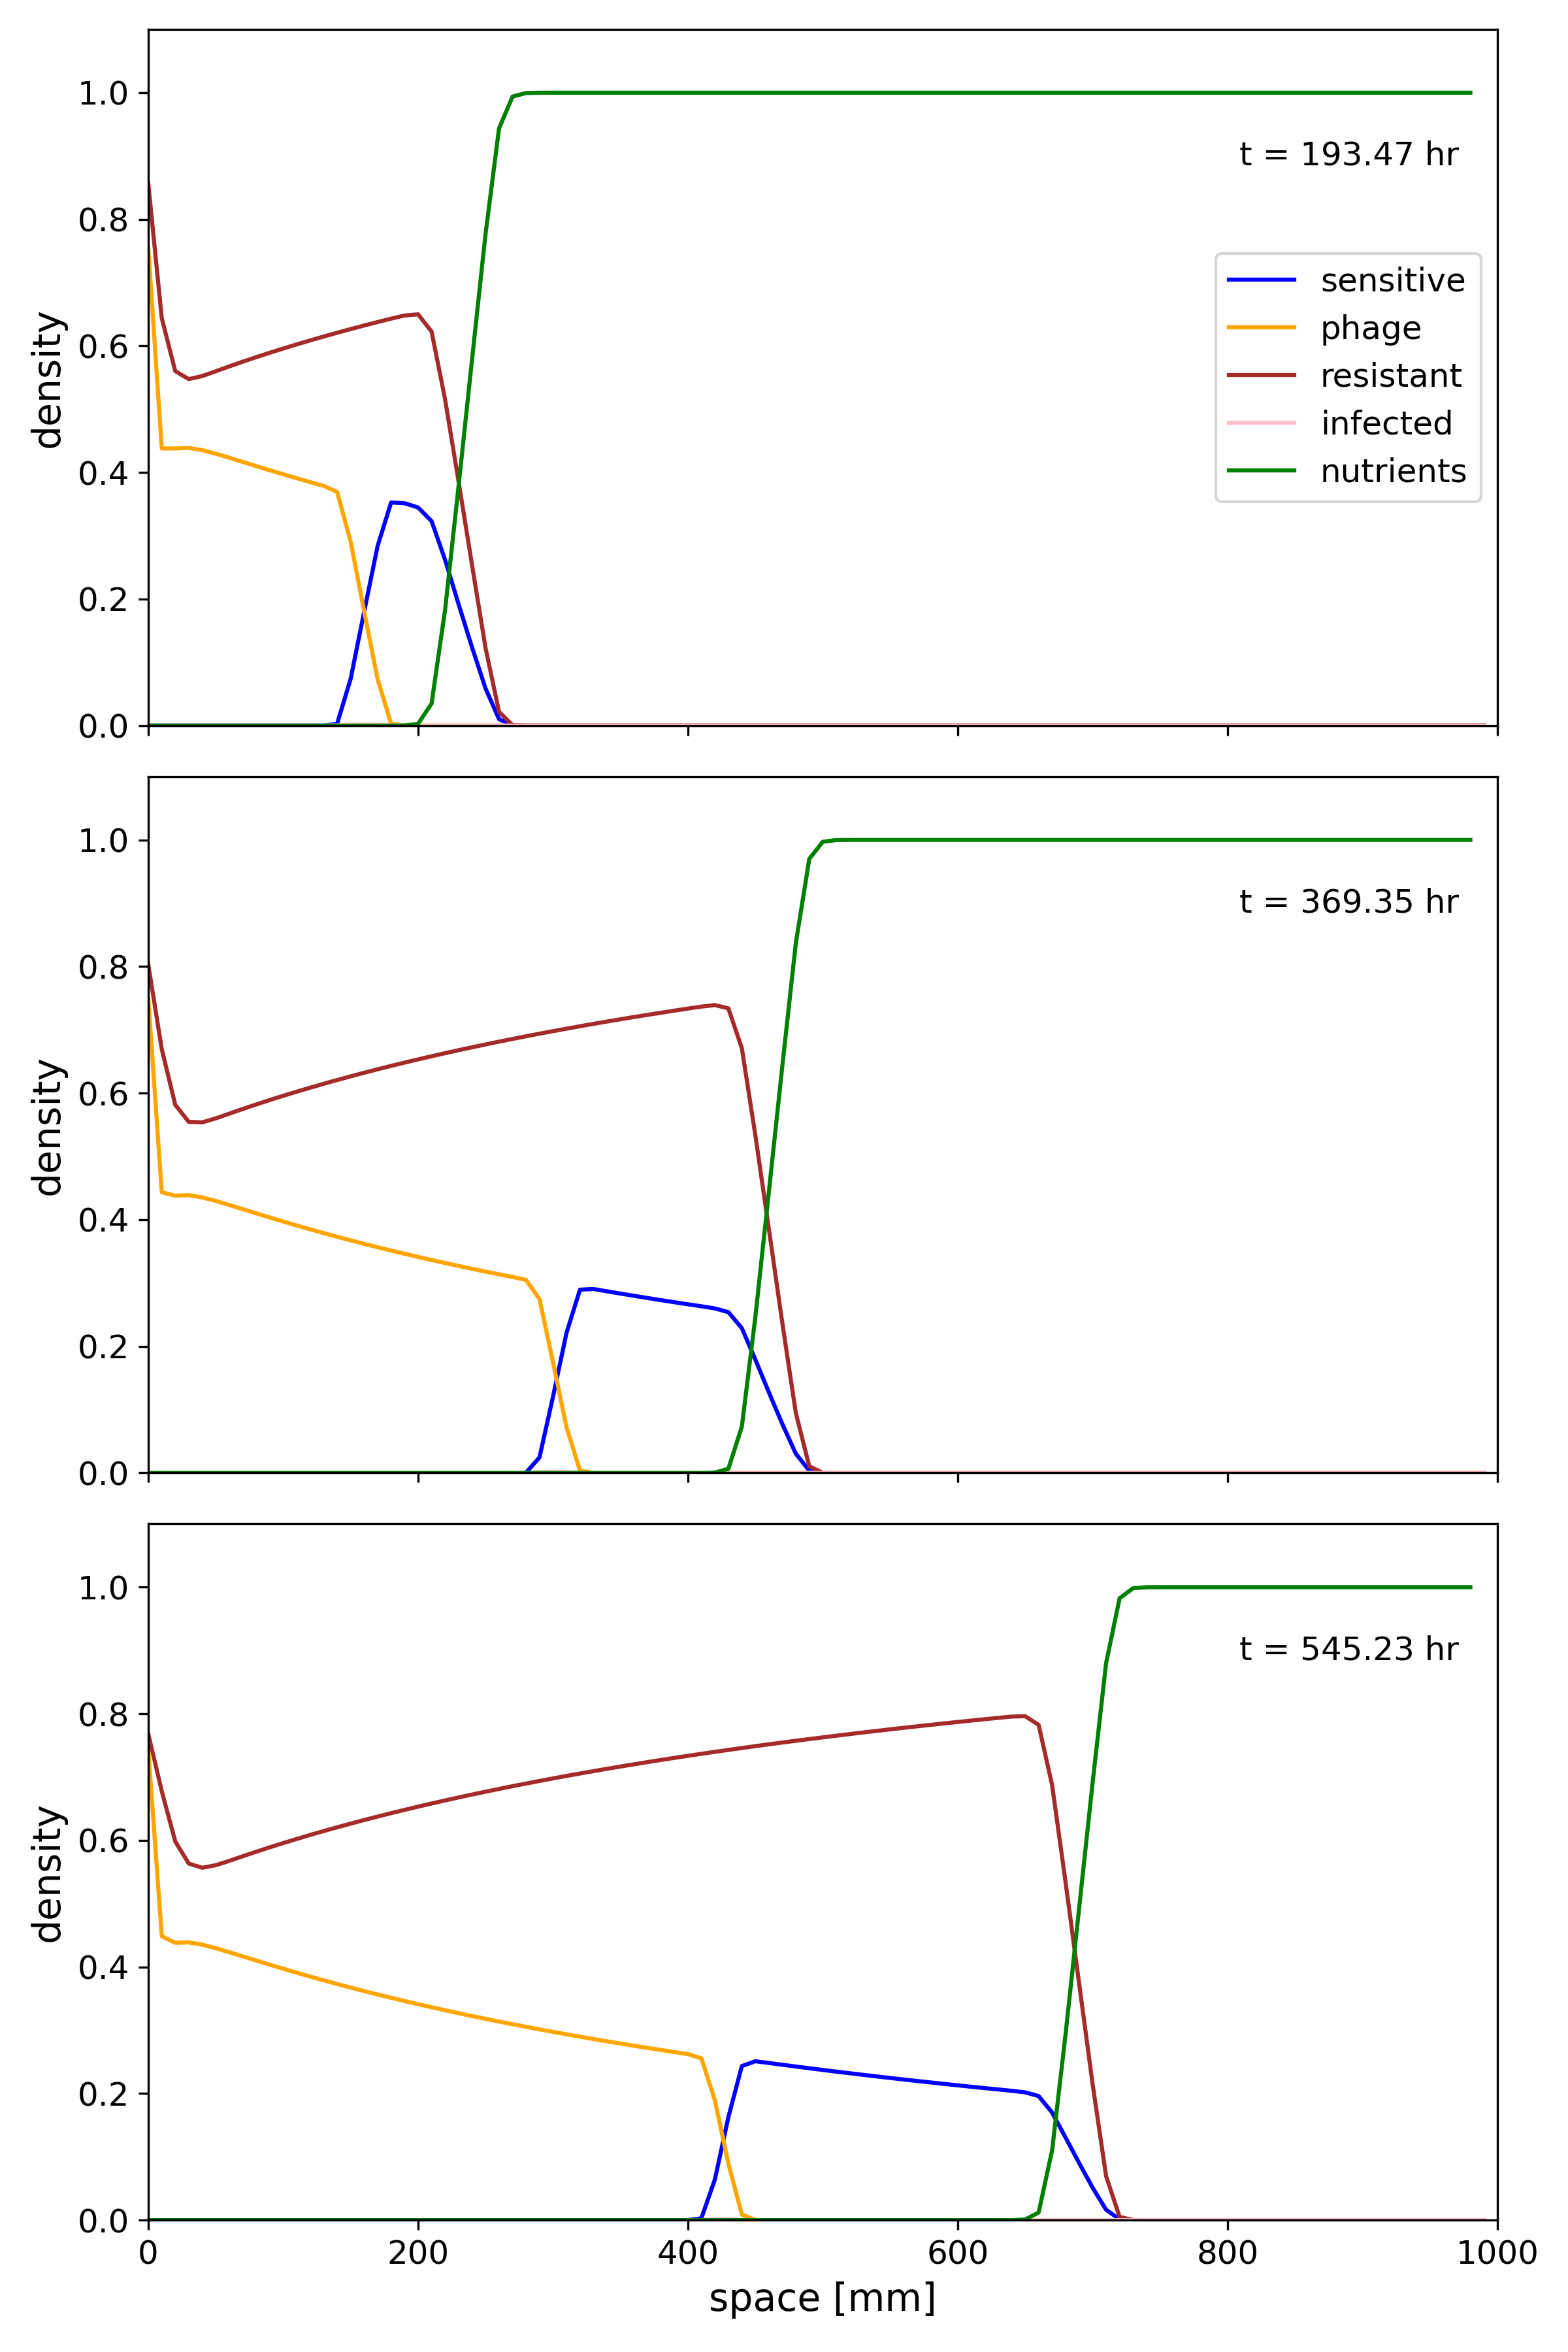
\includegraphics[width=0.9\linewidth]{graphics/2025_09_30_phages_fig6.png}
\caption{\textbf{Time dynamics for a resistant growth rate close to expected transition reveals protective effect for sensitive bacteria} Shown are three time snapshots of the dynamics for $\lambda_r \approx 0.99$, at the peak of protection, revealing widening of the sensitive traveling wave over time, resulting in a higher amount of sensitive bacteria in the system.}
\label{fig:dynamics_peak}
\end{figure}

\section{Widening causes protection}
Looking at the dynamics for the peak protective effect (Figure~\ref{fig:dynamics_peak}), we observe a widening of the sensitive traveling wave over time, resulting in the observed linear increase in amount of sensitive bacteria over time. As the same time, we observe qualitatively a decrease in the height of the sensitive wave. In order to quantify both observations, we increase the resolution around the protective peak (Figure~\ref{fig:results_peak_change_height_width}a) and measure amount (Figure~\ref{fig:results_peak_change_height_width}b), width ((Figure~\ref{fig:results_peak_change_height_width}c) and height ((Figure~\ref{fig:results_peak_change_height_width}d) over time for points around the peak. We clearly see the transition from a plateauing amount ((Figure~\ref{fig:results_peak_change_height_width}b, blue curve) over a linear increasing amount ((Figure~\ref{fig:results_peak_change_height_width}b, gray curve) to a decreasing one (Figure~\ref{fig:results_peak_change_height_width}b, red curve). When studying the height and width, we observe that with increasing resistant growth rate, the sensitive traveling wave transforms from a narrow, high peak to a shallow but wide peak. Once resistant bacteria grow faster, the sensitive traveling wave disappears.

\begin{figure}
\centering
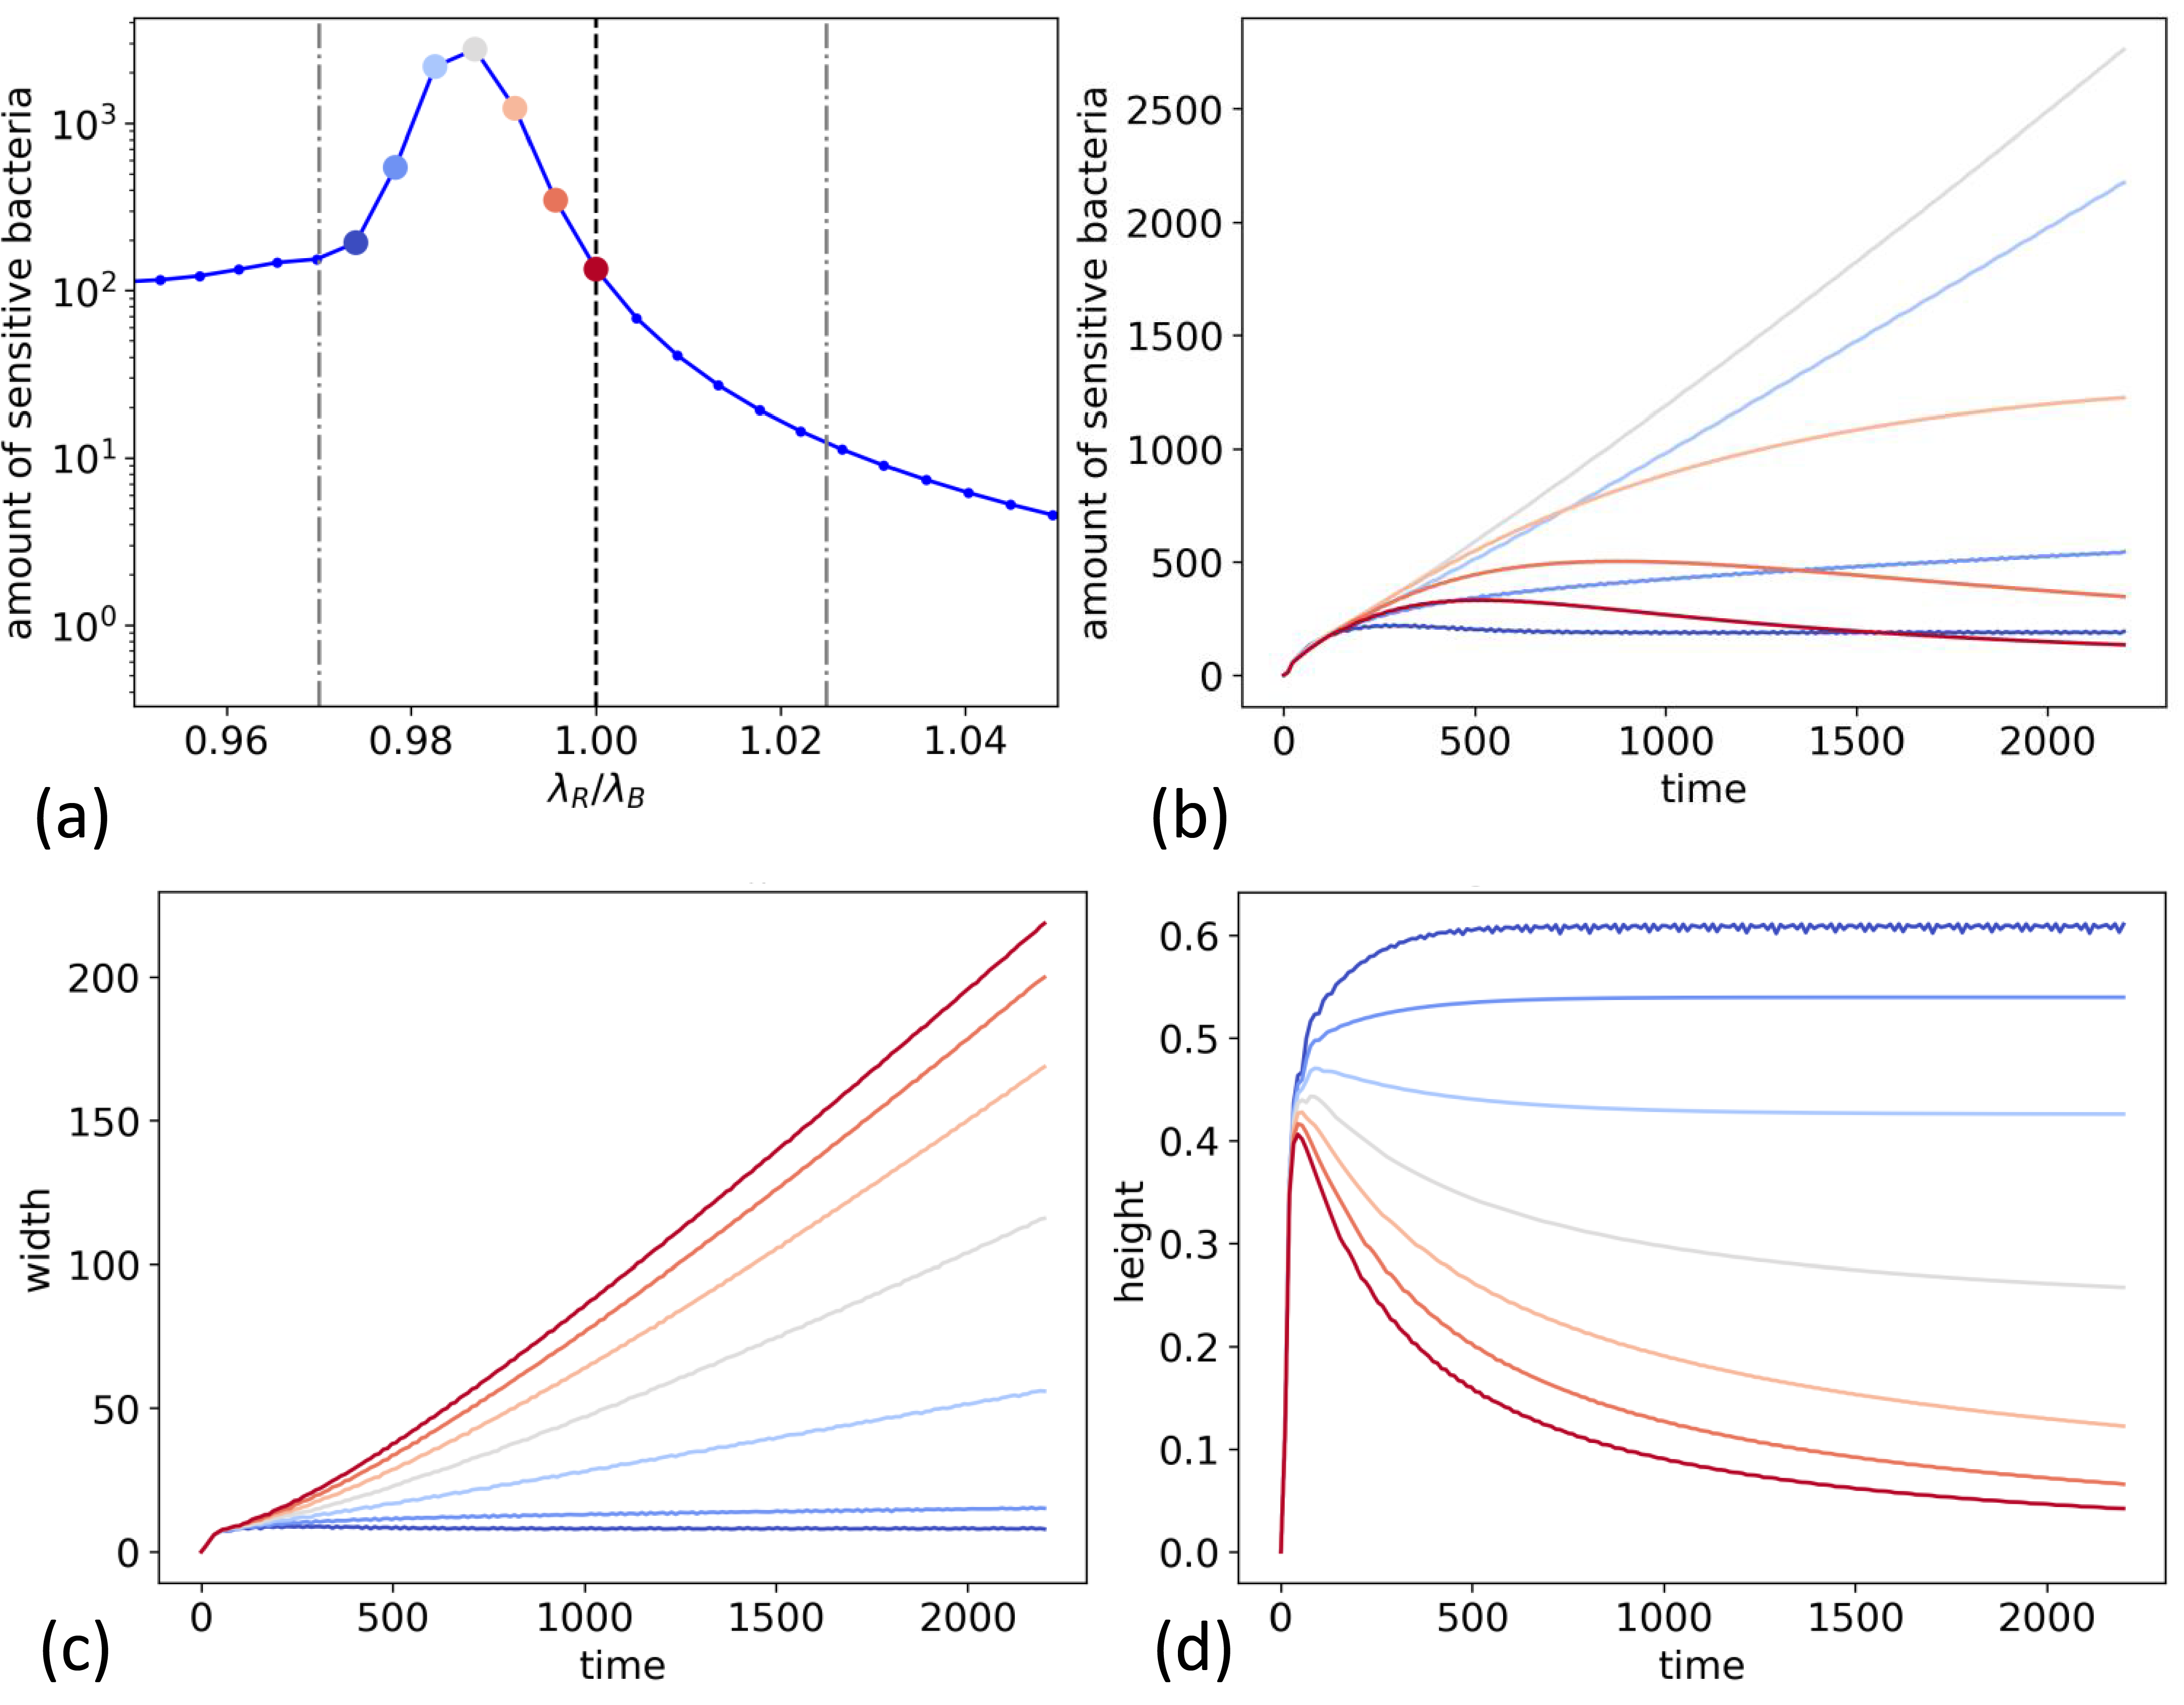
\includegraphics[width=\linewidth]{graphics/2025_09_30_phages_fig7.png}
\caption{\textbf{Closer examination of the protective peak reveals widening} (a) shows a focused, higher resolution, view on the protective peak with color coded markers indicating points around the transition. (b) shows the amount of sensitive bacteria over time for those points around the peak, indicated in (a). (c) and (d) show the width and height over time for these chosen points.}
\label{fig:results_peak_change_height_width}
\end{figure}

\section{Front decoupling results in linear width increase}
The observed linear increase in width over time suggests that the two wave fronts, sensitive bacteria and phages, decouple and travel with constant but different speeds. Indeed, measuring the speeds of these two fronts (Figure~\ref{fig:results_speed_height}a), we observe that the phage front slows down at a lower resistant growth rate than the sensitive bacteria front. Calculating the difference in speed between the two fronts (Figure~\ref{fig:results_speed_height}b, black curve), we observe that the maximal difference is at a higher growth rate than the observed protective effect. However, as is apparent from our previous height and width analysis, for higher growth rates, the peak is diminished and the effect of the widening on the total amount as well. Indeed, when multiplying speed with height as a new quantification of the effect (Figure~\ref{fig:results_speed_height}b, red curve), we observe an effect only for those growth rates which also reveal the protective effect. So overall, the product of speed difference and height explains the observed protective effect. 

\begin{figure}
\centering
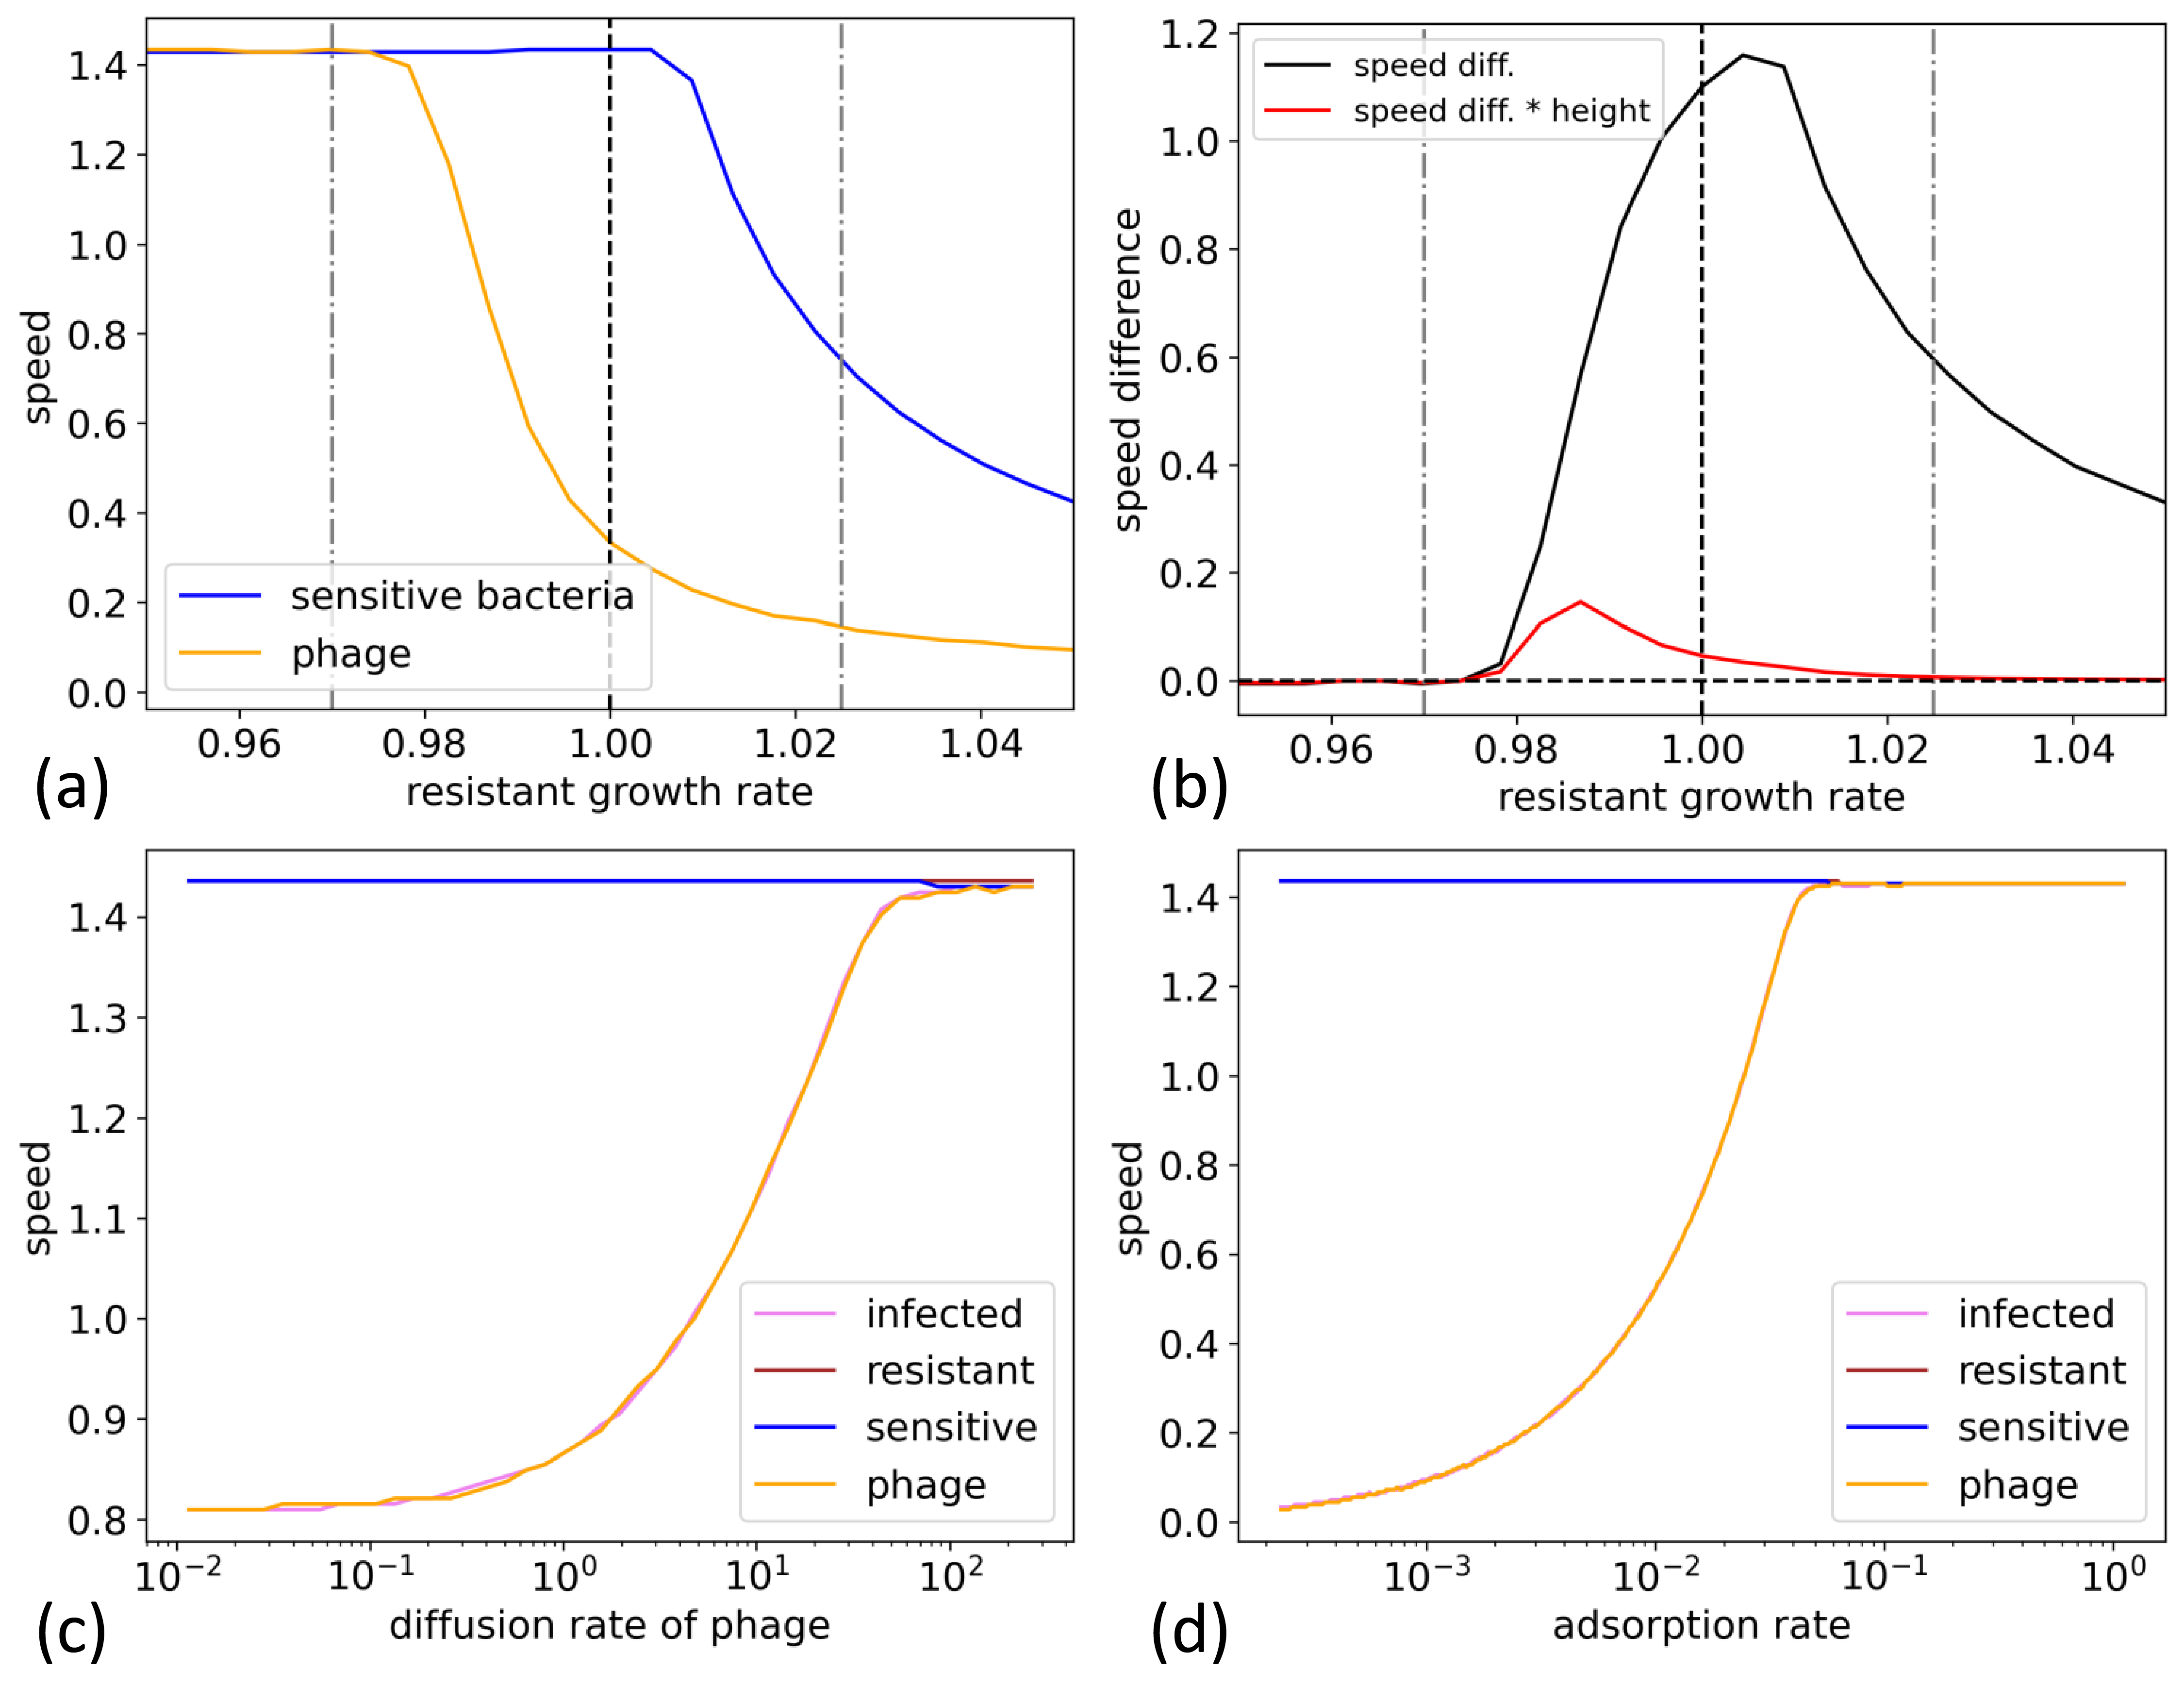
\includegraphics[width=\linewidth]{graphics/2025_09_30_phages_fig8.png}
\caption{\textbf{Speed difference identified as cause for widening} (a) shows the speed of the expanding wave front of phages and of sensitive bacteria as a function of resistant growth rate, (b) shows the difference between these two speeds and the new measurement of the product of speed difference and height}
\label{fig:results_speed_height}
\end{figure}

\section{Nutrient sparsity weakly protects sensitive bacteria from phage infection}
Previous models, studying a phage wave invading an exponentially growing, sensitive population~\cite{Claydon2021-cu} show a separation between the speed of the receding sensitive wave and the speed of the advancing phage wave without resistant bacteria present in the system. Motivated by these results, we are studying in this section, whether we can observe the protective effect in a system without resistant bacteria and thus without nutrient competition when instead limiting the available nutrients directly. Lowering the initially available nutrients in the system, reduces the speed of both waves, phages and bacteria, without a significant difference between those two. Only for a very low nutrient concentration where the height of the sensitive traveling wave is very small, a minor speed difference occurs. This effect is much smaller than the effect obtained when resistant bacteria are present in the system. Hence, we conclude that resistant bacteria are necessary to observe the protective effect.

\section{Impact of diffusion rate of resistant bacteria on protective effect}
Wave speed and bacterial competition are known to depend not only on the growth rate but also on the diffusion rate of the bacteria. Consequently, we analyzed the impact of changes in both of these parameters on the amount of sensitive bacteria while in the analyses before, we focused only on changes in the growth rate and the diffusion rate was equal. We found a clear phase transition from a parameter regime in which sensitive bacteria survive to a parameter regime in which sensitive bacteria do not survive~(Figure~\ref{fig:results_heatmap_effect}). Close to the transition interface, we observe the protective effect. There seems to be a linear correlation between growth rate and diffusion rate for low growth rates, in agreement with the theoretical results for the KPP-equation, describing the speed of a traveling wave as proportional to the square root of the product of growth rate and diffusion rate~\cite{Murray2002-qj, Fisher1937-rd}. However, for higher growth rates, this linear relation collapses and we observe a dominant effect of growth rate rather than diffusion rate. In conclusion, the speed of the resistant traveling wave seems to be the critical parameter enabling the effect rather than changes in the growth rate alone.
\begin{figure}
\centering
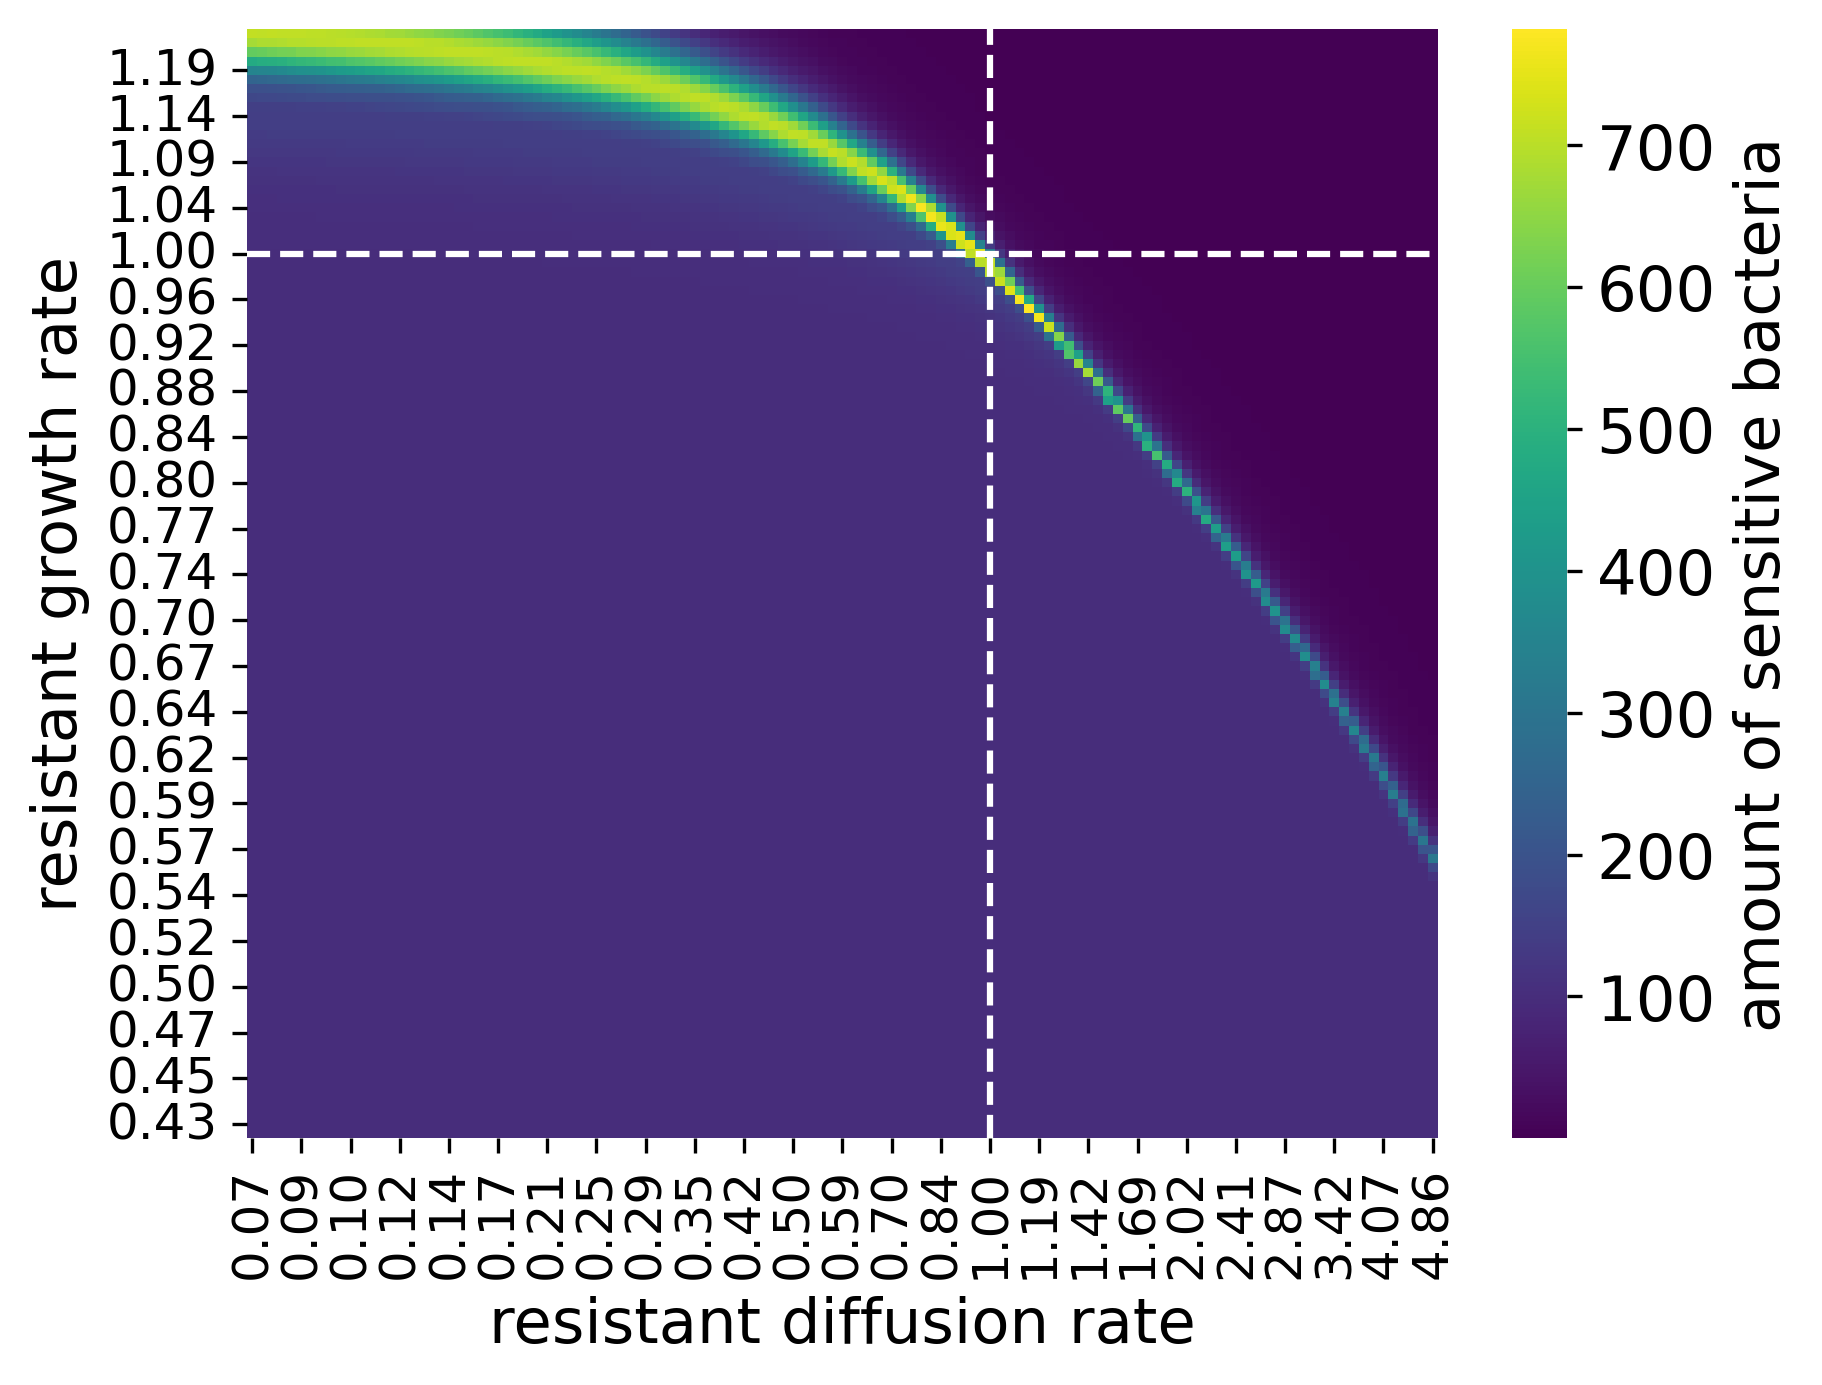
\includegraphics[width=\linewidth]{graphics/2025_09_30_phages_fig9.png}
\caption{\textbf{Phase transition shows protective effect depends on the growth rate and the diffusion rate of resistant bacteria} The heatmap shows the amount of sensitive bacteria for different combinations of resistant growth rate and resistant diffusion rate, indicating a phase transition from a region with sensitive bacteria to a region without. At the interface, we observe an increase in sensitive bacteria.}
\label{fig:results_heatmap_effect}
\end{figure}

\section{Impact of phage properties on bacteria-phage interaction}
Our model includes several fixed parameters, some of which could impact the dynamics. Two of those are standing out, as they are known to directly impact phage speed. In this section, we focus on those two parameters, the phage diffusion rate and the infection rate. While the impact of the first one on the speed is trivial, the impact of the second one was previously observed due to the hitchhiking phenomenon~\cite{Ping2020-vd}. When varying those two parameters, we indeed see a change in phage speed (Figure~\ref{fig:results_parameter_change}). For both parameters, we were able to find scenarios in which decoupling of phage and bacterial waves does not occur.
\begin{figure}
\centering
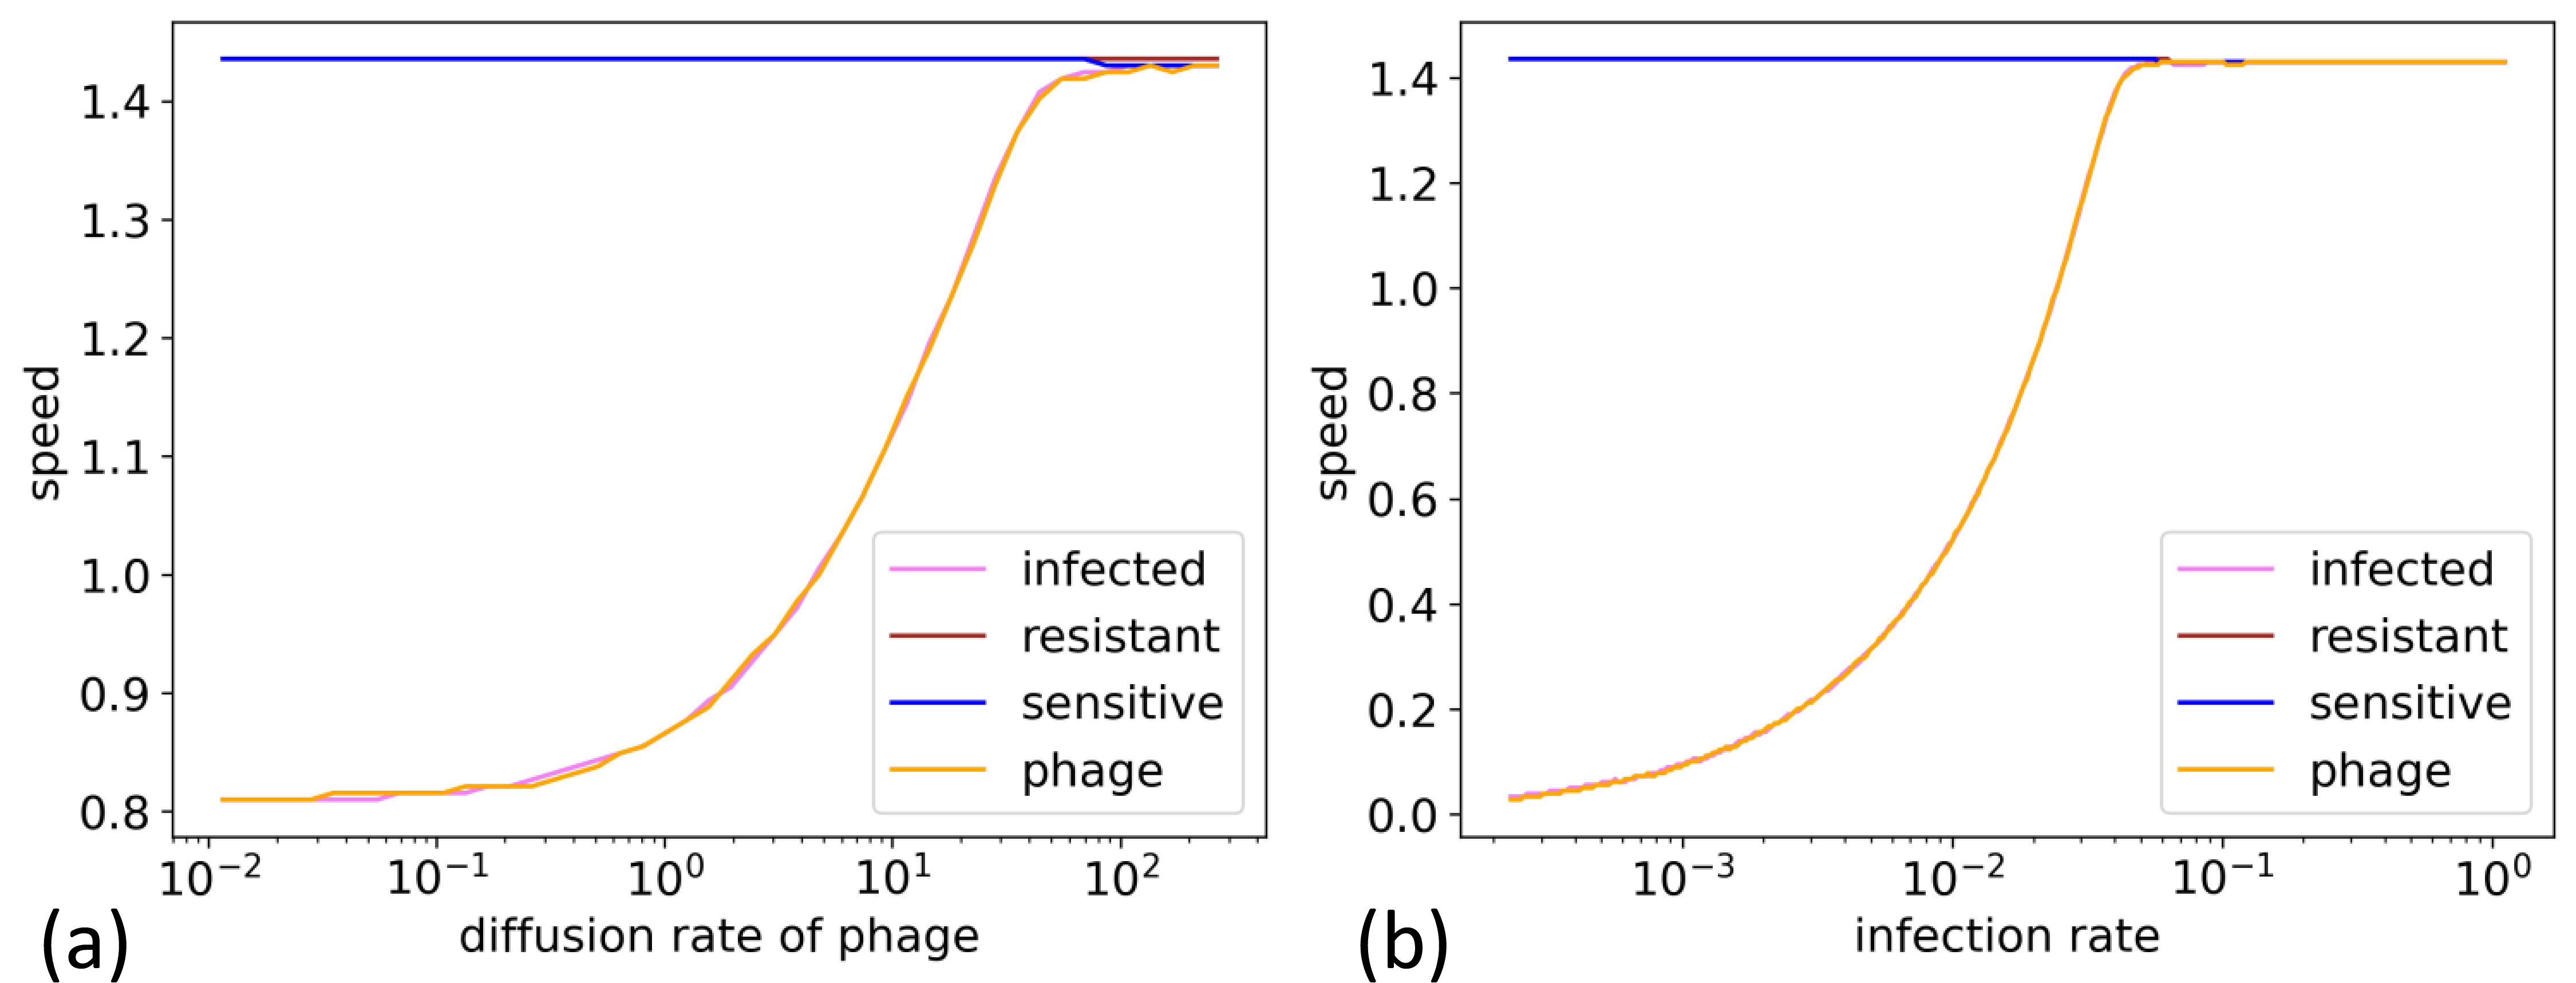
\includegraphics[width=\linewidth]{graphics/2025_09_30_phages_fig10.png}
\caption{\textbf{Changes in phage diffusion rate and infection rate can result in loss of decoupling} (a) shows the impact of phage diffusion rate on the speed of phages and bacteria. While the sensitive bacterial speed is not affected, a higher phage diffusion rate results in a higher phage speed, as expected. (b) shows the impact of the infection rate on the speed and in light of the previously described hitchhiking phenomenon, a higher infection rate and thus more infected bacteria results in a higher phage speed while the sensitive bacterial speed is not affected.}
\label{fig:results_parameter_change}
\end{figure}

\section{Limitations}
Some phages replicate only on growing bacteria due to the dependence on the replication machinery of bacteria~\cite{Los2007-px, Maffei2022-aj}. Hence, we explored such a scenario by limiting the infection rate indirectly through a dependence on the nutrients with:
\begin{equation}
    \eta = \eta_0 \frac{n}{K_n + n}
\end{equation}
where $\eta_0$ is set to be the same infection rate as given in table~\ref{tab:model_parameters}.
In this scenario, we were unable to observe the protective effect and we rather see a phase transition due to fitness of resistant and sensitive bacteria. Furthermore, if comparing it to a no-phage scenario, where bacteria compete without phages in the system, we see only minor differences between these cases.
This means that the ability for phages to replicate on non-growing bacteria is crucial for the protective effect to exist.